\section{DFS and BFS}

%%%%%%%%%%%%%%%
\begin{frame}{Classifying edges}
  \begin{definition}[Classifying edges]
    Given a DFS/BFS traversal $\Rightarrow$ DFS/BFS tree:
    \begin{itemize}
      \item Tree edge: $\to$ child
      \item Back edge: $\to$ ancestor
      \item Forward edge: $\to$ \emph{nonchild} descendant
      \item Cross edge: $\to$ neither ancestor nor descendant
    \end{itemize}
  \end{definition}

  \begin{alertblock}{Remarks:}
    \begin{itemize}
      \item applicable to both DFS and BFS
      \item w.r.t. DFS/BFS trees
    \end{itemize}
  \end{alertblock}
\end{frame}
%%%%%%%%%%%%%%%
\begin{frame}{Classifying edges}
  \begin{exampleblock}{Classifying edges \pno{3.4.1}}
    \begin{figure}
      \begin{subfigure}{0.50\linewidth}
	\centering
	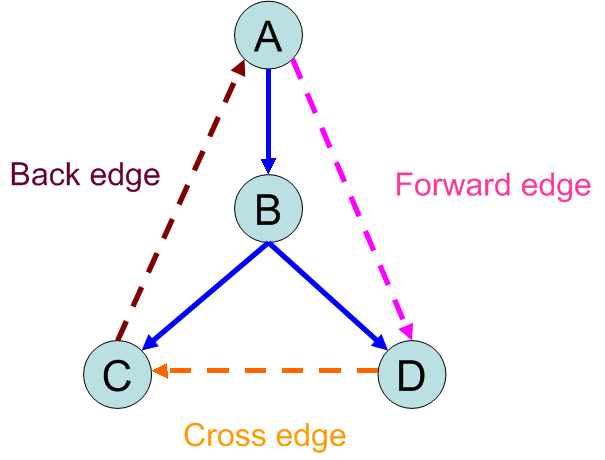
\includegraphics[width=0.50\textwidth]{figures/dfs-digraph.png}
	\caption{DFS on directed graph.}
      \end{subfigure}%
      \begin{subfigure}{0.50\linewidth}
	\centering
	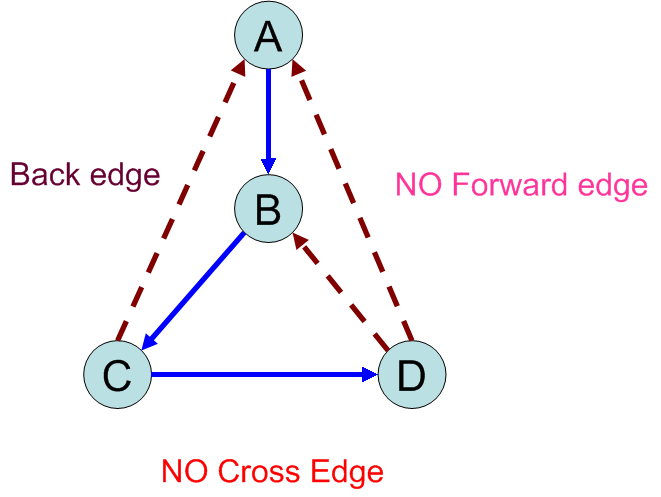
\includegraphics[width=0.50\textwidth]{figures/dfs-undirected.png}
	\caption{DFS on undirected graph.}
      \end{subfigure}

      \begin{subfigure}{0.50\linewidth}
	\centering
	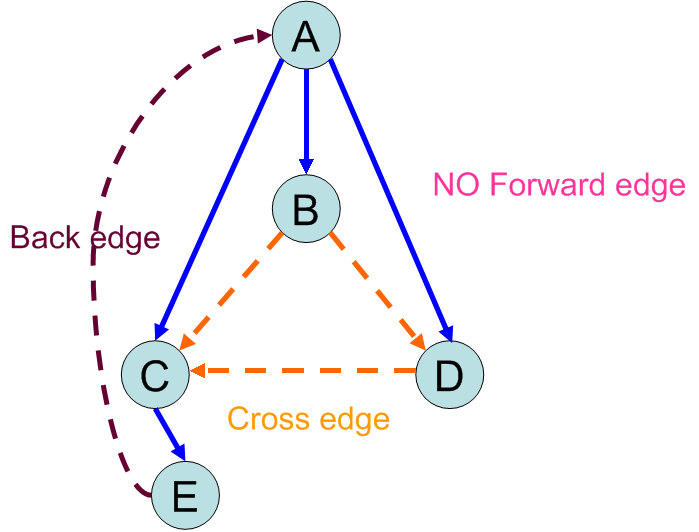
\includegraphics[width=0.50\textwidth]{figures/bfs-digraph.png}
	\caption{BFS on directed graph.}
      \end{subfigure}%
      \begin{subfigure}{0.50\linewidth}
	\centering
	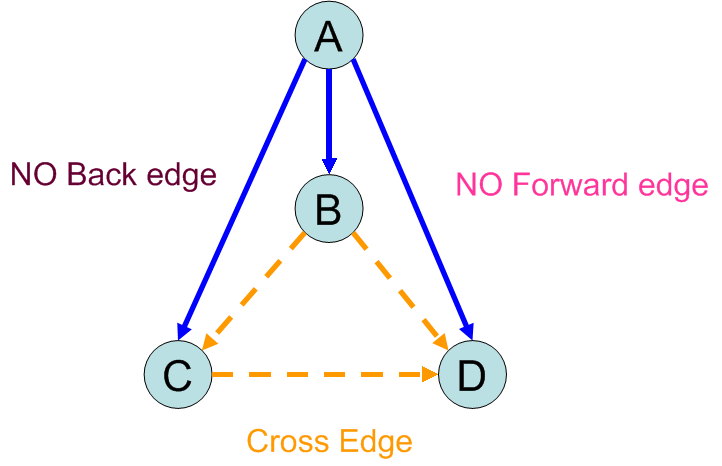
\includegraphics[width=0.60\textwidth]{figures/bfs-undirected.png}
	\caption{BFS on undirected graph.}
      \end{subfigure}
    \end{figure}
  \end{exampleblock}
\end{frame}
%%%%%%%%%%%%%%%
\begin{frame}{Classifying edges}
  \begin{exampleblock}{DFS tree and BFS tree coincide \pno{3.4.30}}
    $G = (V,E), v \in V$. DFS tree $T$ = BFS tree $T'$.

    \begin{itemize}
      \item $G$ is an undirected graph $\Rightarrow$ $G = T$.
      \item $G$ is a digraph $\Rightarrow^{?}$ $G = T$.
    \end{itemize}
  \end{exampleblock}

  \begin{block}{Solution.}
    \begin{itemize}
      \item $T$: tree + back; $T'$: tree + cross
      \item $T$: tree + back + forward + cross; $T'$: tree + back + cross 
    \end{itemize}
  \end{block}
\end{frame}
%%%%%%%%%%%%%%%
\begin{frame}{Distance constraints for BFS}
  \begin{exampleblock}{Distance constraints for BFS \pno{3.4.4}}
    \begin{columns}[t]
      \column{0.40\textwidth}
        BFS on digraph:
	\begin{description}
	  \item[TE:] $d[v] = d[u] + 1$
	  \item[BE:] $0 \le d[v] \le d[u]$
	  \item[CE:] $d[v] \le d[u] + 1$
	\end{description}
      \column{0.60\textwidth}
        BFS on undirected graph:
	\begin{description}
	  \item[TE:] $d[v] = d[u] + 1$
	  \item[CE:] $d[v] = d[u] \lor d[v] = d[u] + 1$ 
	\end{description}
    \end{columns}
  \end{exampleblock}

  \begin{block}{Solution to ``\emph{CE} in BFS on \emph{undirected} graph''.}
    \begin{itemize}
      \item $d[v] = d[u], d[v] = d[u] + 1$
      \item $d[v] < d[u], d[v] > d[u] + 1$
    \end{itemize}
  \end{block}

  \begin{alertblock}{Remark.}
    \begin{itemize}
      \item BFS tree defines a \emph{shortest-path} from its root to every other node.
      \item Layers in BFS on \emph{undirected} graph; c.f. bipartite testing \pno{3.4.26}
    \end{itemize}
  \end{alertblock}
\end{frame}
%%%%%%%%%%%%%%%
\begin{frame}{Lifetime of vertices in DFS}
  \begin{exampleblock}{Lifetime of vertices in DFS \pno{3.4.5}} 
    $\forall u,v$:
    \begin{itemize}
      \item $u$ is an ancestor of $v$: $[\text{d}[v], \text{f}[v]] \subset [\text{d}[u], \text{f}[u]]; [_{u}\; [_{v}\; ]_{v}\; ]_{u}$
      \item $u,v$ has no ancestor/descendant relation: $[\text{d}[v], \text{f}[v]] || [\text{d}[u], \text{f}[u]]$
    \end{itemize}
  \end{exampleblock}

  \begin{block}{Solution.}
    Assume $u, v \in $ DFS tree.

    \begin{itemize}
      \item $c$: least common ancestor of $u,v$ \pno{3.4.17}
      \item $c \to u' \leadsto u; c \to v' \leadsto v$
      \item $u', v'$ disjoint; $u \subset u' \land v \subset v'$
    \end{itemize}
  \end{block}

  \begin{alertblock}{Remark.}
    $\forall u,v: [_{u} \; ]_{u}, [_{v} \; ]_{v}$ \emph{disjoint} $\lor$ \emph{contained} $\Leftarrow$ a ``stack'' view.
  \end{alertblock}
\end{frame}
%%%%%%%%%%%%%%%
\begin{frame}{Preprocessing for ancestor/descendant relation}
  \begin{exampleblock}{Preprocessing for ancestor/descendant relation \pno{3.4.14}}
    \begin{itemize}
      \item binary tree $\Rightarrow$ tree $T$
      \item $r \in T$
    \end{itemize}
  \end{exampleblock}

  \begin{block}{Solution.}
    $v: \text{d}[v], \text{f}[v]$
  \end{block}

  \begin{alertblock}{Remark.}
    $\forall v$: how many descendants?

    $(\text{f}[v] - \text{d}[v] - 1) / 2$
  \end{alertblock}
\end{frame}
%%%%%%%%%%%%%%%
\begin{frame}{Edge types and lifetime of vertices in DFS}
  \begin{exampleblock}{Edge types and lifetime of vertices in DFS \pno{3.4.3}}
    $\forall u \to v$:
    \begin{itemize}
      \item tree/forward edge: $[_{u}\; [_{v}\; ]_{v}\; ]_{u}$
      \item back edge: $[_{v}\; [_{u}\; ]_{u}\; ]_{v}$
      \item cross edge: $[_{v}\; ]_{v}\; [_{u}\; ]_{u}$
    \end{itemize}
  \end{exampleblock}

  \begin{alertblock}{Remark.}
    \begin{itemize}
      \item $\text{f}[v] < \text{d}[u]$: cross edge
      \item $\text{f}[u] < \text{f}[v]$: back edge
    \end{itemize}
  \end{alertblock}
\end{frame}
%%%%%%%%%%%%%%%
